\section{Các yếu tố ảnh hưởng đến chi phí phát triển ứng dụng}

  Chi phí phát triển ứng dụng là một yếu tố quan trọng mà các doanh nghiệp cần cân nhắc kỹ lưỡng trước khi triển khai dự án phần mềm. Trong thực tế, chi phí này không chỉ phụ thuộc vào quy mô hay mục tiêu của sản phẩm, mà còn bị chi phối bởi nhiều yếu tố kỹ thuật và chiến lược khác nhau. Từ đặc điểm của tính năng, kiến trúc hạ tầng, đến vị trí địa lý của đội ngũ phát triển, mỗi yếu tố đều có thể tạo ra sự chênh lệch đáng kể về ngân sách đầu tư. Phần này sẽ trình bày hai nhóm nội dung chính: (1) các yếu tố cốt lõi tác động đến chi phí xây dựng và duy trì ứng dụng, và (2) sự khác biệt về chi phí nhân sự theo khu vực địa lý trên thế giới. Qua đó, doanh nghiệp có thể xác định các điểm cần ưu tiên, tối ưu nguồn lực và lựa chọn chiến lược phát triển phù hợp với điều kiện thực tế của mình.

  
  
% 5.1
\subsection{Các yếu tố chính ảnh hưởng đến chi phí phát triển ứng dụng}
\renewcommand{\labelitemi}{--}  

% https://assets.goodfirms.co/pdfs/how-much-does-it-cost-to-develop-an-app.pdf
  \begin{figure}[H]
    \centering
    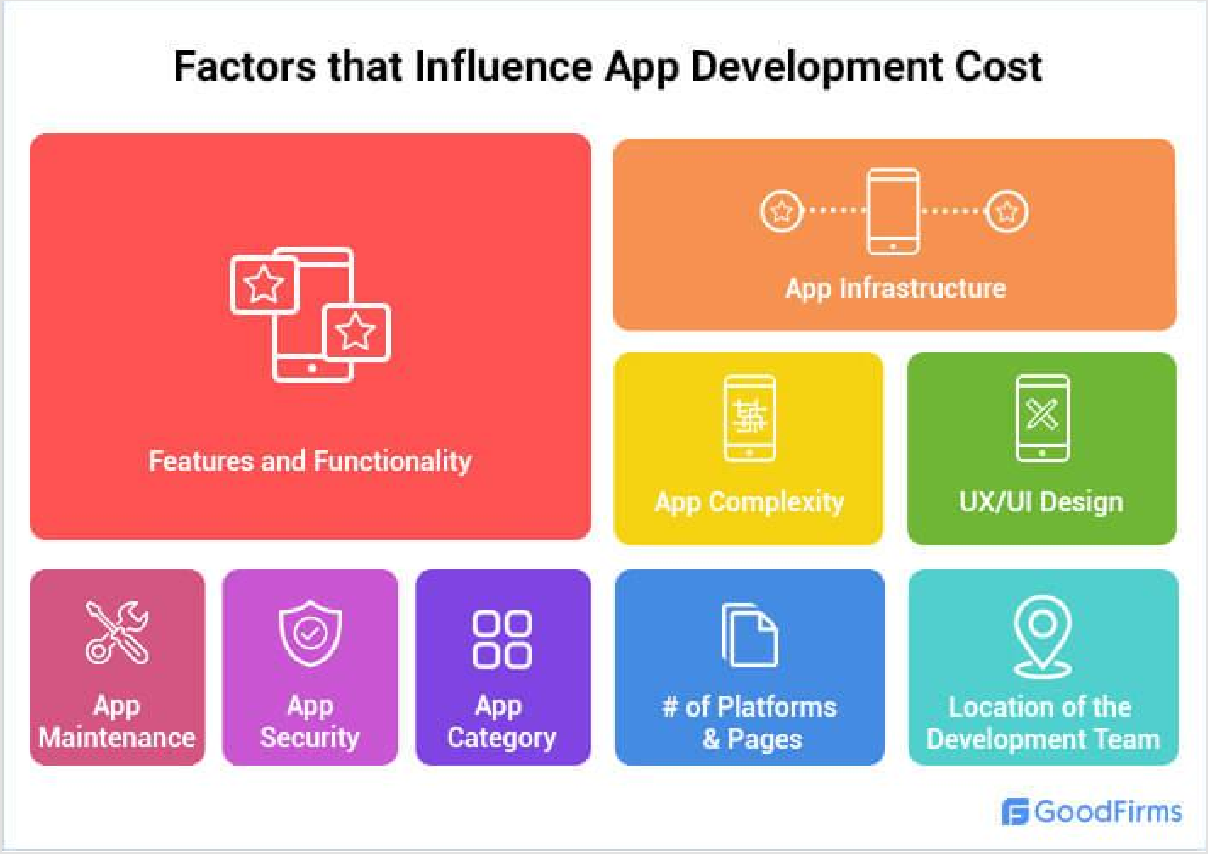
\includegraphics[width=0.6\textwidth]{images/appCosst.png}
    \caption{Các yếu tố chính ảnh hưởng đến chi phí phát triển ứng dụng \cite{goodfirmsAppCost}.}
    \label{fig:fig20}
  \end{figure}

    
      Trong quá trình phát triển ứng dụng, nhiều yếu tố đóng vai trò quyết định đến tổng chi phí, cả trong giai đoạn thiết kế lẫn sau triển khai. Các yếu tố chính bao gồm:
      \setlength{\leftmargini}{1.5cm}
      \begin{itemize}
          \item Tính năng và chức năng (Features and Functionality): Mức độ phức tạp của tính năng tỷ lệ thuận với chi phí phát triển. Ứng dụng có càng nhiều chức năng nâng cao như định vị, livestream, AI tích hợp,… thì đòi hỏi nguồn lực phát triển cao hơn.
          \item Hạ tầng ứng dụng (App Infrastructure): Cách tổ chức hệ thống backend, tích hợp API, hệ thống lưu trữ dữ liệu, bảo mật và tối ưu hiệu năng đều ảnh hưởng lớn đến ngân sách đầu tư. Hạ tầng vững chắc đảm bảo tính ổn định và khả năng mở rộng lâu dài.
          \item Độ phức tạp của ứng dụng (App Complexity): Mức độ phức tạp trong luồng xử lý nghiệp vụ và logic kinh doanh đòi hỏi thời gian phân tích và phát triển dài hơn, từ đó làm tăng chi phí.
          \item Thiết kế trải nghiệm người dùng (UX/UI Design): Giao diện càng trực quan, hiện đại, và thân thiện thì cần đầu tư nhiều thời gian hơn cho thiết kế và kiểm thử.
          \item Chi phí bảo trì (App Maintenance): Sau khi triển khai, ứng dụng cần cập nhật thường xuyên để vá lỗi, cải tiến tính năng hoặc thích nghi với nền tảng mới.
          \item Yêu cầu bảo mật (App Security): Ứng dụng xử lý dữ liệu nhạy cảm (ngân hàng, y tế, tài chính...) đòi hỏi mức độ bảo mật cao, từ đó làm tăng chi phí đầu tư.
          \item Loại ứng dụng (App Category): Tùy thuộc vào lĩnh vực hoạt động (thương mại điện tử, chăm sóc sức khỏe, mạng xã hội…), mức độ phức tạp và chi phí phát triển sẽ khác nhau.
          \item Số lượng nền tảng và màn hình (Number of Platforms \& Pages): Ứng dụng hỗ trợ nhiều nền tảng như iOS, Android, Web với giao diện đa dạng sẽ phát sinh thêm chi phí thiết kế và kiểm thử.
          \item Vị trí nhóm phát triển (Location of the Development Team): Chi phí nhân công thay đổi theo từng khu vực địa lý. Các nhóm tại Mỹ hoặc Tây Âu thường có chi phí cao hơn so với châu Á.
      \end{itemize}
    \vspace{0.5em}

    
      Trong số các yếu tố trên, kiến trúc hạ tầng phần mềm (App Infrastructure) đóng vai trò then chốt:
      \setlength{\leftmargini}{1.5cm}
      \begin{itemize}
          \item Đây là “xương sống” kỹ thuật của toàn bộ hệ thống, quyết định tính ổn định, bảo mật, khả năng tích hợp API, cloud và cơ sở dữ liệu.
          \item Nếu được thiết kế tốt ngay từ đầu, hạ tầng giúp giảm đáng kể chi phí bảo trì và tránh rủi ro gián đoạn trong quá trình vận hành.
      \end{itemize}
    \vspace{0.5em}

% 5.2
\subsection{Chi phí thuê nhân sự theo khu vực địa lý}

\begin{table}[ht]
  \centering
  \begin{tabular}{|p{3.2cm}|c|c|c|c|}
  \hline
  \textbf{Title of Employee} & \textbf{United States} & \textbf{Latin America} & \textbf{Eastern Europe} & \textbf{Asia} \\
  \hline
  Business Analyst    & \$110 -- \$205 & \$45 -- \$55 & \$40 -- \$63 & \$30 -- \$42 \\
  Architect           & \$198 -- \$292 & \$60 -- \$72 & \$50 -- \$77 & \$35 -- \$48 \\
  Project Manager     & \$133 -- \$233 & \$55 -- \$66 & \$45 -- \$70 & \$35 -- \$48 \\
  Jr. Developer       & \$105 -- \$111 & \$35 -- \$44 & \$25 -- \$42 & \$18 -- \$24 \\
  Mid-Level Dev & \$132 -- \$140 & \$30 -- \$52 & \$35 -- \$49 & \$25 -- \$34 \\
  Sr. Developer       & \$154 -- \$163 & \$45 -- \$55 & \$45 -- \$70 & \$30 -- \$42 \\
  Lead Developer      & \$176 -- \$187 & \$50 -- \$61 & \$45 -- \$70 & \$35 -- \$50 \\
  Junior QA           & \$77 -- \$81   & \$30 -- \$39 & \$25 -- \$42 & \$20 -- \$30 \\
  Mid-Level QA        & \$99 -- \$105  & \$35 -- \$44 & \$30 -- \$48 & \$25 -- \$32 \\
  Senior QA           & \$143 -- \$169 & \$40 -- \$51 & \$35 -- \$60 & \$30 -- \$40 \\
  Graphic Designer    & \$79 -- \$163  & \$40 -- \$50 & \$35 -- \$56 & \$25 -- \$36 \\
  \hline
  \end{tabular}
  \caption{Mức lương cho các vai trò nhân viên khác nhau trên khắp các khu vực \cite{rubygarageWebCost}.}
  \label{tab:salary-comparison}
  \end{table}
  
\renewcommand{\labelitemi}{--}    
    
        Một trong những yếu tố quan trọng ảnh hưởng đến tổng chi phí phát triển phần mềm chính là chi phí thuê nhân sự theo khu vực địa lý. Các công ty phần mềm, đặc biệt là những doanh nghiệp quốc tế hoặc các dự án có nhu cầu thuê ngoài (outsourcing), thường căn cứ vào mức chi phí trung bình theo giờ làm việc của các vai trò chuyên môn trong ngành công nghệ thông tin để ra quyết định tuyển dụng. Dữ liệu trong bảng ở phần trên được tổng hợp từ 4 khu vực tiêu biểu trên toàn cầu gồm United States (Hoa Kỳ), Latin America (Mỹ Latin), Eastern Europe (Đông Âu) và Asia (Châu Á). Mỗi khu vực có mức chi phí khác nhau rõ rệt, phản ánh sự chênh lệch về mức sống, kỹ năng lao động cũng như nhu cầu thị trường. Thống kê này bao phủ 12 vai trò phổ biến trong các dự án phát triển phần mềm hiện nay, giúp đưa ra cái nhìn tổng quan về chi phí nhân sự theo từng nhóm chức năng.
    \vspace{0.5em}

    
      Đối với nhóm Quản lý và Thiết kế Kiến trúc, mức chi phí thuê nhân sự được ghi nhận là cao nhất trong tất cả các vai trò. Nhóm này bao gồm ba vị trí chủ chốt: Business Analyst (chuyên viên phân tích nghiệp vụ), Architect (kiến trúc sư phần mềm), và Project Manager (quản lý dự án). Trong đó, kiến trúc sư phần mềm đóng vai trò xây dựng khung nền kỹ thuật, đảm bảo hệ thống có thể mở rộng và vận hành ổn định; còn chuyên viên phân tích nghiệp vụ đóng vai trò cầu nối giữa khách hàng và nhóm kỹ thuật; trong khi quản lý dự án là người điều phối toàn bộ tiến độ và tài nguyên. Tại Hoa Kỳ, mức giá thuê cho các vị trí này có thể lên tới gần \$300/giờ – một con số phản ánh tầm quan trọng chiến lược và yêu cầu chuyên môn cao. Mức chi phí này giảm dần tại các khu vực khác, với Latin America và Eastern Europe dao động ở mức trung bình, còn Asia (Châu Á) là nơi có mức chi phí thấp nhất, chỉ từ \$30 – \$48/giờ. Điều này khiến các công ty quốc tế thường ưu tiên thuê ngoài nhóm nhân sự cấp cao từ khu vực châu Á để tiết kiệm chi phí nhưng vẫn đảm bảo hiệu quả.
    \vspace{0.5em}

    
      Tiếp theo là nhóm Lập trình viên (Developer), một trong những thành phần cốt lõi tạo nên sản phẩm phần mềm. Nhóm này được chia nhỏ theo cấp độ kinh nghiệm, bao gồm: Junior Developer, Mid-Level Developer, Senior Developer và Lead Developer. Sự phân loại này phản ánh mức độ độc lập, độ phức tạp của nhiệm vụ mà mỗi cấp độ có thể đảm nhiệm, cũng như ảnh hưởng đến tiến độ và chất lượng sản phẩm. Mức chi phí thuê sẽ tăng tương ứng với cấp độ, từ Junior đến Lead Developer. Tại các khu vực phát triển như Hoa Kỳ, mức lương của Senior hoặc Lead Developer có thể gần tương đương với nhóm kiến trúc sư. Trong khi đó, các khu vực như Latin America hay Eastern Europe có mức chi phí trung bình, phù hợp cho các công ty tầm trung. Asia tiếp tục là khu vực có lợi thế về chi phí, khi mức thuê nhân sự lập trình ở mọi cấp độ đều ở mức thấp hơn đáng kể, giúp các doanh nghiệp tiết kiệm ngân sách mà vẫn có thể tiếp cận với nguồn lực kỹ thuật chất lượng nếu tuyển chọn kỹ lưỡng.
    \vspace{0.5em}

    
      Trong chu trình phát triển phần mềm, kiểm thử phần mềm (QA) là khâu đảm bảo chất lượng đầu ra trước khi triển khai chính thức. Nhóm QA cũng được chia theo cấp độ kinh nghiệm, bao gồm: Junior QA, Mid-Level QA, và Senior QA. So với Developer hoặc Architect, mức chi phí thuê QA thường thấp hơn, nhưng vẫn có sự chênh lệch rõ rệt giữa các khu vực. Tại Mỹ, một Senior QA có thể nhận mức thù lao lên đến \$169/giờ – thậm chí cao hơn Mid-Level Developer tại cùng khu vực (khoảng \$140/giờ). Điều này cho thấy, tại các thị trường phát triển, việc kiểm thử phần mềm được đánh giá rất cao và đòi hỏi kỹ năng chuyên môn sâu. Tại châu Á, các vai trò QA được thuê với mức giá thấp hơn đáng kể, giúp tiết kiệm đáng kể chi phí cho các công ty đang hướng đến tự động hóa kiểm thử hoặc mở rộng nhóm QA.
    \vspace{0.5em}

    
      Cuối cùng là vai trò thiết kế giao diện (Graphic Designer), vốn không yêu cầu chuyên môn kỹ thuật quá sâu như lập trình nhưng vẫn đóng vai trò quan trọng trong việc tạo ra trải nghiệm người dùng hấp dẫn và nhất quán. Tại các thị trường phát triển như Mỹ, chi phí thuê designer vẫn ở mức khá cao do đòi hỏi về thẩm mỹ, khả năng sử dụng công cụ thiết kế chuyên nghiệp và phối hợp chặt chẽ với nhóm phát triển sản phẩm. Trong khi đó, các khu vực như Đông Âu hay châu Á có chi phí thuê thấp hơn đáng kể, đặc biệt phù hợp với các dự án cần thiết kế giao diện ở mức cơ bản đến trung cấp. Việc lựa chọn graphic designer từ các khu vực này giúp doanh nghiệp duy trì ngân sách ở mức hợp lý mà vẫn đảm bảo tính thẩm mỹ và hiệu quả trong giao diện người dùng.
    \vspace{0.5em}

    
      Tóm lại, chi phí thuê nhân sự phát triển phần mềm có sự biến động lớn theo từng khu vực địa lý và vai trò cụ thể. Việc hiểu rõ mức giá trung bình theo giờ và sự khác biệt giữa các nhóm chuyên môn sẽ giúp doanh nghiệp đưa ra chiến lược thuê nhân sự hiệu quả hơn, cân bằng giữa chi phí và chất lượng. Trong bối cảnh toàn cầu hóa và sự phát triển mạnh mẽ của mô hình làm việc từ xa, các công ty hoàn toàn có thể tối ưu hóa nguồn lực bằng cách kết hợp nhân sự ở các khu vực khác nhau, tận dụng lợi thế chi phí của khu vực châu Á và chất lượng kỹ thuật cao từ các khu vực khác để xây dựng đội ngũ phát triển linh hoạt và hiệu quả.
